\section{Pipeline de Renderizado Programable}
La función del pipeline de renderizado es generar imágenes bidimensionales para ser desplegadas en pantalla dada una cámara virtual, objetos tridimensionales, fuentes de luz, ecuaciones sombreado, texturas y otros \cite{Akenine-Moller:2002:RR:553838}. Este pipeline está divido en varias etapas como se observa en la Figura \ref{fig:pipeline_rendering}.
\begin{figure}[H]
	\centering
	\includegraphics[width=\linewidth]{media/pipeline_rendering.pdf}
	\caption{Etapas del pipeline de renderizado.}
	\label{fig:pipeline_rendering}
\end{figure}
\subsection{Procesador de Vértices}
El procesador de vértices o \emph{vertex shader} realiza operaciones sobre los vértices que definen a la geometría a renderizar. Un vértice puede estar definido por sus coordenadas en el espacio tridimensional u otra información como color, vector normal, características para la iluminación, coordenadas de texturas, entre otros.
\subsection{Procesador de Geometría}
El procesador de geometría o \emph{geometry shader} es una capacidad reciente en la \ac{GPU}. Esta etapa del pipeline permite la manipulación de las mallas que representan la geometría en escena por primitiva. De esta forma los vértices de entrada al pipeline pueden ser enviados al \emph{geometry shader} como vértices individuales, líneas (dos vértices) o triángulos (tres vértices). El \emph{geometry shader} permite la modificación de los parámetros que definen estas primitivas y la generación de nuevas primitivas que serán enviadas al proceso de rasterización.
\subsection{Rasterización}
Las primitivas que alcanzan esta etapa del pipeline son procesadas por la unidad de rasterización en la \ac{GPU}. En esta etapa todos los polígonos son escaneados y convertidos en valores dentro de una cuadrícula regular bidimensional. Durante esta conversión, el triángulo es configurado para generar todos los fragmentos que cubren el área de proyección de este triángulo. Luego por cada uno de estos fragmentos se calculan sus propiedades como color, posición y coordenadas de textura u otros utilizando interpolación lineal entre estas propiedades almacenadas en los tres vértices del triángulo procesado. Los fragmentos generados son luego enviados al procesador de fragmentos.
\subsection{Procesador de Fragmentos}
Todos los fragmentos generados durante el proceso de rasterización son procesados en el procesador de fragmentos o \emph{fragment shader}. Durante este proceso se realizan operaciones como mapeo de texturas, cálculo de iluminación por fragmento y otras técnicas de sombreado. Estos fragmentos luego de ser procesados son escritos en un \emph{framebuffer} y enviados al hardware para ser procesados según operaciones de visibilidad y mezclado para finalmente ser mostrados en pantalla.
\subsection{Cómputo de Propósito General en la GPU}
La \ac{GPU} está diseñada específicamente para el renderizado de gráficos en computadora. Esta puede procesar de forma independiente muchos vértices y fragmentos en paralelo. En este sentido la \ac{GPU} es un procesador de flujo de datos que puede operar en paralelo ejecutando un núcleo o \emph{kernel} sobre los registros en este flujo. Con las nuevas capacidades de cómputo en las GPU se ha incrementado la flexibilidad de estos procesadores, agregando nuevas operaciones y permitiendo su uso para programación de propósito general. Ello facilita el uso de la GPU como un procesador de cómputo paralelo masivo utilizando los muchos núcleos o \emph{cores} de cómputo existentes en las GPU modernas. Esta técnica es llamada \ac{GPGPU}.

\section{Técnicas en Renderizado de Imágenes}

En esta sección se explican técnicas comunes utilizadas en síntesis o renderizado de imágenes que son relevantes para este trabajo.

\subsection{Mapeado de Sombras}
\label{subsec:shadowmapping}
Con la luz representada en forma de rayos las superficies sombreadas reciben menos rayos de luz, ya que estas están ocluidas por otras superficies que se encuentra entre ellas y los emisores de luz. En el pipeline de renderizado estándar, donde las superficies en escenas son representadas en geometría poligonal, trazar rayos por cada fragmento para comprobar la visibilidad del mismo no es una operación trivial.

Los mapas de sombras, presentados inicialmente por Lance Williams en 1978 \cite{Williams:78} son una solución simple para el cálculo de visibilidad de un fragmento. La técnica consiste en proyectar la escena en una textura bidimensional desde la posición y con la dirección de una fuente de luz. La proyección es calculada utilizando una matriz de proyección $P_{l}$. Por cada píxel de esta textura la profundidad de cada fragmento sobre una superficie es almacenada. Esta textura es llamada mapa de sombra.

Una vez que se procede a renderizar la escena desde el punto de vista del observador, por cada fragmento con posición $p_{ws}$ en espacio de mundo, la posición en el mapa de sombra $p_{sh}$ es calculada utilizando la siguiente ecuación:
\begin{equation}
    p_{sh} = P_{l} \cdot p_{ws}
    \label{eq:p_to_shadowmap}
\end{equation}
\begin{figure}[H]
	\centering
	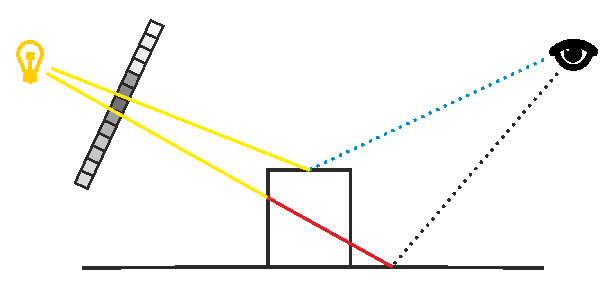
\includegraphics[width=0.80\linewidth]{media/shadow_mapping.eps}
	\caption{La profundidad almacenada en el mapa de sombra (amarillo) es comparada con la profundidad del punto en la superficie desde la luz (rojo).}
	\label{fig:shadow_mapping}
\end{figure}
Como se muestra en la Figura \ref{fig:shadow_mapping}, si la profundidad del fragmento desde la fuente de luz es mayor que el valor almacenado en el mapa de sombra entonces este punto está sombreado.

El mapeado de sombras es una solución sencilla y efectiva al problema de pruebas de visibilidad pero esta técnica tiene dos mayores desventajas. El mapa de sombras está limitado por la resolución de la textura y además este representa una discretización de la profundidad de la escena vista desde la fuente de luz, lo que introduce una variedad de anomalías visuales. A partir de este concepto existe una variedad de algoritmos para el cálculo de sombras que intentan solventar estos problemas u obtener resultados de mejor calidad visual.

\subsection{Sombreado Diferido}
\label{sub:deferred_rendering_theory}
En sombreado directo la representación poligonal de la escena es rasterizada y operaciones por píxel como iluminación y sombreado son realizadas por cada fragmento generado por el proceso de rasterización. Esto es poco efectivo cuando se toma en consideración que muchos fragmentos no forman parte de la imagen final.

Con sombreado diferido se pueden realizar estas operaciones por píxel solo sobre los fragmentos visibles. Este concepto está basado en el trabajo de Deering et al. en 1998 \cite{Deering:1988}. La escena es renderizada solo una vez y varios atributos de la escena son almacenados en buffers. Este buffer es llamado \ac{GBuffer} y fue introducido por Saito et al. en 1990 \cite{Saito:1990}. El contenido general de un G-Buffer es profundidad, albedo y normal (ver Figura \ref{fig:gbuffer}). Esto puede cambiar según las necesidades de la aplicación. El propósito de almacenar esta información es separar las operaciones que solo son necesarias sobre los fragmentos visibles de la rasterización de toda la escena, de manera que cálculos como iluminación ahora son realizados en otro paso solo sobre cada píxel almacenado en el \ac{GBuffer}.

\begin{figure}[H]
	\centering
	\begin{subfigure}[t]{0.32\textwidth}
		\centering
		\captionsetup{justification=centering}
		\includegraphics[width=\linewidth]{media/engine-Context2-Texture13level0.png}
		\caption*{Normales.}
	\end{subfigure}%
	\hspace{0.01\textwidth}
	\begin{subfigure}[t]{0.32\textwidth}
		\centering
		\captionsetup{justification=centering}
		\includegraphics[width=\linewidth]{media/engine-Context2-Texture14level0.png}
		\caption*{Albedo.}
	\end{subfigure}%
	\hspace{0.01\textwidth}
	\begin{subfigure}[t]{0.32\textwidth}
		\centering
		\captionsetup{justification=centering}
		\includegraphics[width=\linewidth]{media/engine-Context2-Texture17level0.png}
		\caption*{Profundidad.}
	\end{subfigure}%
	\caption{El contenido de un buffer de geometría.}
	\label{fig:gbuffer}
\end{figure}

\subsection{Voxelización}
\label{sec:voxelization}
Un vóxel o a veces llamado píxel volumétrico representa una muestra singular o elemento volumétrico sobre un grid regular en un espacio tridimensional. Este vóxel puede contener cualquier valor definido por la aplicación o incluso múltiples valores. 

El proceso de generar superficies discretas en una representación volumétrica a través de vóxeles se le llama voxelización (ver Figura \ref{fig:rigid_grid}).

\begin{figure}[H]
	\centering
	\begin{subfigure}{0.33\textwidth}
		\centering
		\includegraphics[width=.6\linewidth]{media/rigid01.pdf}
		\captionsetup{width=0.95\textwidth}
		\caption{Grid regular del vóxeles.}
	\end{subfigure}%\\
	\begin{subfigure}{0.33\textwidth}
		\centering
		\includegraphics[width=.6\linewidth]{media/rigid02.pdf}
		\captionsetup{width=0.95\textwidth}
		\caption{Superficie en el grid.}
	\end{subfigure}%\\
	\begin{subfigure}{0.33\textwidth}
		\centering
		\includegraphics[width=.6\linewidth]{media/rigid03.pdf}
		\captionsetup{width=.95\textwidth}
		\caption{Superficie en vóxeles.}
	\end{subfigure}%
	\caption{Representación de una superficie en vóxeles con voxelización fina.}
	\label{fig:rigid_grid}
\end{figure}

Se puede distinguir el proceso de voxelización de superficies en dos clases: voxelización fina con separabilidad factor 6 y voxelización conservativa con todos los vóxeles que tocan la superficie activos o separabilidad factor 26. En el trabajo de Huang et al. en 1998 \cite{Huang:1998:AMV:288126.288181} se describe el proceso de voxelización y terminología con mayor detalle. También existen cuatro tipos de enfoques en voxelización:

\begin{itemize}
	\label{list:voxelization_types}
	\item \textbf{Voxelización binaria:} Cada vóxel sólo almacena si hay geometría presente o no.
	\item \textbf{Voxelización multi-valor:} Cada vóxel puede almacenar múltiples valores de data arbitraria como opacidad, normal, etc.
	\item \textbf{Voxelización de contorno:} Sólo se voxeliza la superficie o contorno de los objetos.
	\item \textbf{Voxelización sólida:} Además de la superficie también se voxeliza el interior del objeto.
\end{itemize}
